\chapter*{Introduction}

\addcontentsline{toc}{chapter}{Introduction}

This work deals with the mathematical modeling of fluid flow with a focus on finding the optimal shape of walls, particularly in the issue of total cavopulmonary connection. In many engineering fields such as the automotive or aerospace industries, incorporating optimization processes to find the optimal shape of the studied object is common practice. However, in the field of clinical medicine, for various reasons, the use of optimization techniques is still not so common. To obtain relevant results, it is necessary to model the complex blood flow inside often complicated geometries as accurately as possible using thoroughly tested methods. Validation of numerical simulation results against measured data is also often complicated, as performing experiments \textit{in vivo} (in a living organism) is naturally very difficult, sometimes even impossible.

Nevertheless, the process of shape optimization can find great potential especially in cardiac and vascular surgery \cite{Abraham2005, Weddell2015, Marsden2008}. Developing an optimization process usable in the medical environment would provide doctors with an \textit{in vitro} (outside a living organism) way to assess surgical procedures within patient-specific geometries. Designing and implanting objects such as stents or artificial valves would then be directly tailored to the patient's anatomy, which can lead to improved clinical outcomes, reduced risk of postoperative complications, and a general improvement in the patient's quality of life after the procedure \cite{Marsden2008}.

An example of a specific surgical procedure where the process of wall shape optimization can find its application is the so-called total cavopulmonary connection (\textit{TCPC}). TCPC is performed in children diagnosed with a so-called functionally single ventricle, i.e., in patients with a severe congenital heart defect, due to which their heart can effectively utilize only one functional ventricle, and in whom it is not possible to surgically ensure a functioning two-ventricle circulation \cite{Chaloup}. It is a surgery in which the superior vena cava (\textit{vena cava superior}, labeled \textit{d} in Fig.~\ref{fig:tcpc}) is surgically connected to the pulmonary artery. The inferior vena cava (\textit{vena cava inferior}, labeled \textit{b} in Fig.~\ref{fig:tcpc}) is also connected directly to the pulmonary artery (\textit{arteria pulmonalis}, labeled \textit{a} in Fig.~\ref{fig:tcpc}), usually using a so-called extracardiac conduit (labeled \textit{c} in Fig.~\ref{fig:tcpc}), or extracardiac channel, created from a vascular prosthesis \cite{Rubtsova, Delorme}.

\begin{figure}[h]
	\centering
	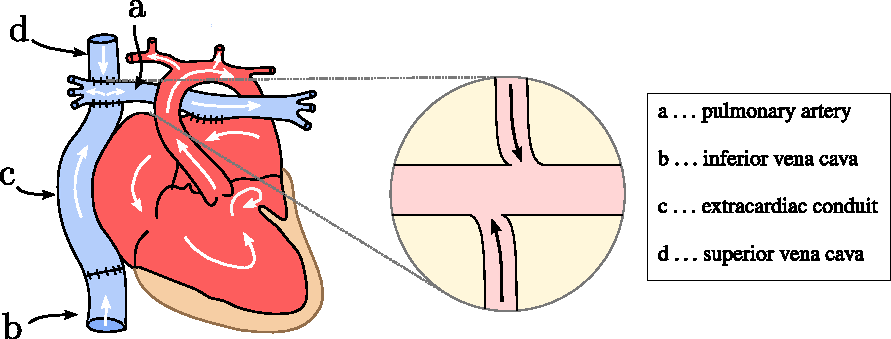
\includegraphics[width=0.97\textwidth]{figures/heart.pdf}
	\vspace{5mm}
	\caption{Diagram of the total cavopulmonary connection. The enlarged section shows the site of the extracardiac conduit connection.}
	\label{fig:tcpc}

\end{figure}

TCPC allows the creation of a functional blood circulation; however, the resulting circulatory system is specific and sensitive to several factors that undesirably contribute to energy loss in the system. This gradually leads to the overall failure of the system. These are mainly the influences of turbulent flow and collision of flows, which occur, for example, at the outlets of the superior and inferior vena cava into the pulmonary artery. The issue of optimal connection of the extracardiac conduit for the purpose of minimizing energy loss or minimizing tissue stress can be the subject of the optimization process \cite{Chaloup, vanBake, Wang}. There are a number of studies dealing with the design of the optimal shape of the conduit connection; however, they often rely only on the trial-and-error method and do not use optimization methods \cite{Rijnberg2018, Porfiryev2020, Tang2014}.

To create an optimization framework usable for cardiac surgery when simulating blood flow, it is necessary to use an efficient and reliable numerical method to compute the values of the objective function, which is subject to minimization. In this work, we use the lattice Boltzmann method (\textit{LBM}) for numerical computations. Note that for the LBM, a code developed at the Department of Mathematics of FNSPE CTU in Prague was used and modified according to the needs of this work. The main advantage of LBM is the possibility of massive parallelization on GPUs (graphics processing units), thanks to which computations take orders of magnitude less time than standard numerical methods used for modeling fluid flow \cite{PE, Kruger}. On the other hand, a significant disadvantage of LBM in terms of boundary geometry is that it uses a regular grid for spatial discretization. This presents a significant problem in the context of this work, as the boundaries of the bodies being modeled or the boundaries of vessels are discretized in a stair-step manner. Therefore, part of this work and the previous bachelor's thesis \cite{JB} is devoted to the study and implementation of interpolated boundary conditions, which allow the actual shape of the boundary of the modeled bodies to be taken into account within the discretization. Due to the use of these boundary conditions, even a small change in the shape of the geometry used in the numerical simulation leads to a change in the result obtained by the numerical simulation; therefore, within optimization, gradient optimization methods can be used, for example.

The structure of the work is as follows. The first chapter focuses on the mathematical model of fluid flow with an emphasis on modeling blood flow in vessels. The second chapter discusses the numerical method LBM in detail. In the third chapter, the tool developed for efficient parameterization and subsequent automatic geometry generation is further discussed. The fourth chapter contains the theory of mathematical optimization and the optimization methods used in this work; moreover, the proposed optimization framework is presented in this chapter. The last chapter presents the results of the numerical simulations performed. First, the functionality of the used optimization framework is tested on a series of designed test problems with one optimization parameter. Then, optimization is tested on more complex problems with multiple optimization parameters, and among other things, the influence of the optimization method used and the choice of the initial solution estimate is examined. One of the more complex problems includes a simplified 2D model of a vascular junction arising in total cavopulmonary connection.



